\documentclass{beamer}

\title[MO433 - Unsupervised Learning]{MO433 - Unsupervised Learning \\ \textcolor{red}{Introduction to Unsupervised Learning}} 
\author{Alexandre Xavier Falc{\~{a}}o}
\institute[IC-UNICAMP]{Institute of Computing - UNICAMP}
\date{afalcao@ic.unicamp.br}

\begin{document}

\begin{frame}
\titlepage
\end{frame}

\begin{frame}{Agenda}

\begin{itemize}
\item What is unsupervised learning?
\vspace{0.5cm}
\item The importance of the joint \alert{probability density function} (pdf, distribution for simplicity).
\vspace{0.5cm}
\item Overview of this course with emphasis on deep generative models.
\vspace{0.5cm}
\item Basic concepts from Probability and Information Theory. 
\end{itemize}

\end{frame}

\begin{frame}{What is unsupervised learning?}
Let $\mathbf{x}=(x_1,x_2,\ldots,x_n)\in \mathbb{R}^n$ be a random
vector, whose variables $x_i$, $i\in [1,n]$, are observations
describing different measures of a phenomenon under study.
\pause \vspace{0.5cm} Such variables might be:
\begin{itemize}
  \item age, income, purchase frequency to discover customers with
    similar characteristics;
    \vspace{0.3cm}
  \item expression levels of different genes to find co-regulated gene
    groups or genes that express together;
    \vspace{0.3cm}
  \item latent features from input images to synthesize new images; etc.
\end{itemize}

\pause \vspace{0.5cm} \alert{Unsupervised learning} is the process of
discovering the underlying structure (clusters, associations, latent
factors) of a joint pdf $p(\mathbf{x})$ from $N$
observed samples
$\{\mathbf{x}^{(1)},\mathbf{x}^{(2)},\ldots,\mathbf{x}^{(N)}\}$,
without access to labeled target variables.
\end{frame}

\begin{frame}{The importance of $p(\mathbf{x})$}
  \begin{itemize}
  \item Knowledge of $p(\mathbf{x})$ allows data analysis, synthesis, and efficient
    annotation by focusing human effort on more representative samples from high-density regions.
\pause \vspace{0.3cm}    
  \item It enables better classification by utilizing the joint
    pdf $p(\mathbf{x},y) =
    P(y\mid\mathbf{x})p(\mathbf{x})$ rather than only the conditional
    probability $P(y\mid\mathbf{x})$ represented by standard classifiers.
\begin{center}  
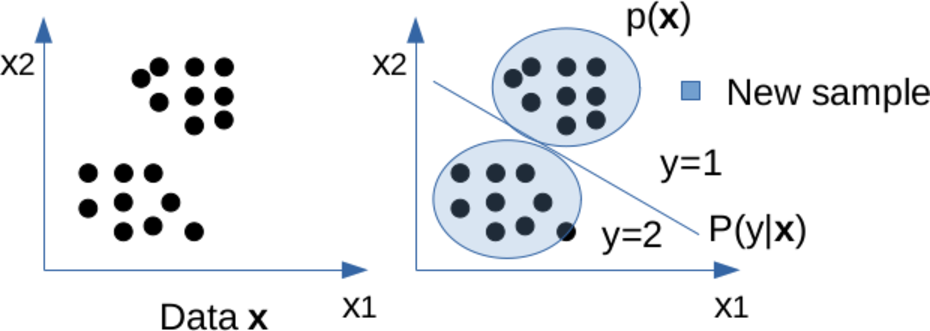
\includegraphics[scale=0.45]{./figs/joint_distribution_classification.pdf}
\end{center}
Samples in regions with low $p(\textbf{x})$ could remain unclassified.
\pause \vspace{0.3cm}    
  \item This is particularly valuable for handling class imbalance,
    outlier detection, and uncertainty quantification.
  \end{itemize} 
\end{frame}
  
\begin{frame}{What will you learn in this course?}

\begin{itemize}
  \item \textbf{Mathematical Foundations} — as needed to support core models and algorithms.
  \vspace{0.3cm}
  \item \textbf{Dimensionality Reduction \& Visualization} — uncover patterns and structure in high-dimensional data.
  \vspace{0.3cm}
  \item \textbf{Clustering \& Distribution Estimation} — learn methods to group data and model its probability structure.
  \vspace{0.3cm}
  \item \textbf{Representation Learning} — with autoencoders, contrastive and non-contrastive self-supervised methods.
  \vspace{0.3cm}
  \item \textbf{Deep Generative Models} — create realistic images with deep neural architectures.
\end{itemize}

\end{frame}
  
\begin{frame}{Main Types of Deep Generative Models}
Deep generative models aim to estimate the underlying pdf \(
p(\mathbf{x}) \) to generate new, realistic samples.

\vspace{0.3cm}
\begin{itemize}
  \item \textbf{Autoregressive Models} \\
  Factorize the joint pdf as a sequence of conditional distributions:  
  \( p(\mathbf{x}) = \prod_{i=1}^n p(x_i \mid x_{<i}) \). \\
  \textit{Examples: PixelCNN, GPT.}
  
  \vspace{0.3cm}
  \item \alert{\textbf{Latent Variable Models}} \\
  Introduce hidden variables \( \mathbf{z} \) and marginalize them out:  
  \( p(\mathbf{x}) = \int_{-\infty}^{+\infty} p(\mathbf{x} \mid \mathbf{z}) p(\mathbf{z}) \, d\mathbf{z} \) \\
  \textit{Examples: VAEs, GANs, stable diffusion}.

  \vspace{0.3cm}
  \item \textbf{Flow-based Models} \\
  Use invertible bijective vector-valued functions \( \mathbf{f} \) between latent space and data: \(\mathbf{x} =  \mathbf{f}(\mathbf{z}) \), so   
  \( p(\mathbf{x}) = p(\mathbf{z}) \left| \det \left(\frac{\partial \mathbf{f}^{-1}}{\partial \mathbf{x}}\right) \right| \). \\
  \textit{Examples: RealNVP, Glow.}
\end{itemize}
\end{frame}

\begin{frame}{Other Generative Modeling Approaches}

Alternative methods use implicit or non-likelihood-based estimation techniques to model \( p(\mathbf{x}) \):

\vspace{0.3cm}
\begin{itemize}
  \item \textbf{Energy-Based Models} \\
  Assign an energy score \( \mathcal{E}(\mathbf{x}) \) and define distribution as:  
  \( p(\mathbf{x}) = \frac{1}{Z} \exp(-\mathcal{E}(\mathbf{x})) \), with \( Z = \sum_{\mathbf{x}} \exp\{-\mathcal{E}(\mathbf{x})\}\). \\
  \textit{Examples: Deep Boltzmann machines}.

  \vspace{0.3cm}
  \item \textbf{Score-Based Models} \\
  Estimate the gradient of log-density \( \nabla_{\mathbf{x}} \log p(\mathbf{x}) \), and use it in Langevin dynamics or reverse-time stochastic differential equation to sample data. \\
  \textit{Examples: Score-based diffusion models, noise conditional score network}.
\end{itemize}

\vspace{0.3cm}
Each model type balances tractability, generation speed, training stability, and sample realism.

\end{frame}

\begin{frame}{More Details About This Course}

\vspace{0.3cm}
The course is under preparation and all essential course resources will be available online, including:

\vspace{0.5cm}
\begin{itemize}
  \item Lecture slides.
  \vspace{0.4cm}
  \item Student evaluation criteria.
  \vspace{0.4cm}
  \item Downloadable datasets.
  \vspace{0.4cm}
  \item Recommended bibliography.
  \vspace{0.4cm}
  \item Additional reference materials and updates
\end{itemize}

\vspace{0.8cm}
\begin{center}
\textbf{Visit:} \url{www.ic.unicamp.br/~afalcao/mo433}
\end{center}
\end{frame}

\begin{frame}{Random variables}
  Let $x$ be a continuous random variable, then its mean $E[x]$ and variance $\text{Var}[x]$ are defined by
  \begin{eqnarray*}
    E[x] & = & \mu = \int_{-\infty}^{+\infty} x p(x) \, dx \\
    \text{Var}[x] & = & E[(x-\mu)^2] = \sigma^2 = \int_{-\infty}^{+\infty} (x-\mu)^2 p(x) \, dx
  \end{eqnarray*}
  where $p(x)$ is the pdf of $x$.\\
  \vspace{0.5cm}
  Let $\bar{x} = \frac{x_1 + x_2 + \ldots + x_n}{n}$ be the sample mean of $n$ independent random variables.

\textbf{Sample mean properties:}
\begin{eqnarray*}
E[\bar{x}] &=& \frac{E[x_1]+E[x_2]+\ldots+E[x_n]}{n} \\
\text{Var}[\bar{x}] &=& \frac{\text{Var}[x_1]+\text{Var}[x_2]+\ldots+\text{Var}[x_n]}{n^2}
\end{eqnarray*}  
\end{frame}

\begin{frame}{Central Limit Theorem}
\textbf{Classical CLT (i.i.d. case):}
If $x_1, x_2, \ldots, x_n$ are independent and identically distributed with $E[x_i] = \mu$ and $\text{Var}[x_i] = \sigma^2$, then:
$$\frac{\bar{x} - \mu}{\sigma/\sqrt{n}} \xrightarrow{d} N(0,1) \text{ as } n \to \infty$$
where $\bar{x} = \frac{x_1 + x_2 + \ldots + x_n}{n}$ and:
\begin{eqnarray*}
E[\bar{x}] &=& \mu \\
\text{Var}[\bar{x}] &=& \frac{\sigma^2}{n}
\end{eqnarray*}
\textbf{Generalized CLT:}
Even if $x_i$ have different distributions, under certain regularity conditions (e.g., Lindeberg condition: no single variance dominates), the standardized sum still converges to a normal distribution -- i.e., $\bar{x}\sim N(\mu,\frac{\sigma^2}{n})$ -- with pdf:
$$p(\bar{x}) = \frac{\sqrt{n}}{\sqrt{2\pi}\sigma} \exp\left(-\frac{n(\bar{x}-\mu)^2}{2\sigma^2}\right)$$
\end{frame}

\begin{frame}{Statistical dependency}
For two random variables, $x_1$ and $x_2$, the joint pdf:
\begin{eqnarray*}
p(x_1,x_2) &=& p(x_1\mid x_2)p(x_2) = p(x_2\mid x_1)p(x_1)
\end{eqnarray*}

\textbf{Marginalization:}
\begin{eqnarray*}
p(x_1) &=& \int_{-\infty}^{+\infty} p(x_1,x_2) \, dx_2 = \int_{-\infty}^{+\infty} p(x_1\mid x_2)p(x_2) \, dx_2 \\
p(x_2) &=& \int_{-\infty}^{+\infty} p(x_1,x_2) \, dx_1 = \int_{-\infty}^{+\infty} p(x_2\mid x_1)p(x_1) \, dx_1
\end{eqnarray*}

\textbf{Independence:} $x_1$ and $x_2$ are independent if and only if:
\begin{eqnarray*}
p(x_1,x_2) &=& p(x_1)p(x_2); p(x_1\mid x_2) = p(x_1); \mbox{and }p(x_2\mid x_1) = p(x_2)
\end{eqnarray*}

\textbf{Dependence:} If $x_1$ and $x_2$ are dependent, then knowing one variable provides information about the other.
\end{frame}


\begin{frame}{Statistical dependency}
\textbf{Covariance:}
\begin{eqnarray*}
\text{Cov}(x_1,x_2) &=& E[(x_1-\mu_1)(x_2-\mu_2)] \\
&=& \int_{-\infty}^{+\infty}\int_{-\infty}^{+\infty}(x_1-\mu_1)(x_2-\mu_2)p(x_1,x_2) \, dx_1 \, dx_2
\end{eqnarray*}
where $\text{Cov}(x_1,x_2) = 0$ when $x_1$ and $x_2$ are independent (\alert{uncorrelated}).

\vspace{0.5cm}
\textbf{Correlation coefficient:} 
\begin{eqnarray*}
\rho_{x_1x_2} &=& \frac{\text{Cov}(x_1,x_2)}{\sigma_{x_1}\sigma_{x_2}}
\end{eqnarray*}
where $|\rho_{x_1x_2}| \leq 1$ and $|\text{Cov}(x_1,x_2)| \leq \sigma_{x_1}\sigma_{x_2}$ (\alert{Cauchy-Schwarz Inequality}).
\end{frame}

\begin{frame}{Entropy}
  Entropy measures \alert{uncertainty} (how hard it is to predict) in
  \textbf{bits} (number of yes/no questions needed to guess the
  outcome).
\begin{eqnarray*}
H(x_1) &=& -\int_{-\infty}^{+\infty} p(x_1) \log p(x_1) \, dx_1 \\
H(x_2) &=& -\int_{-\infty}^{+\infty} p(x_2) \log p(x_2) \, dx_2 \\
H(x_1,x_2) &=& -\int_{-\infty}^{+\infty} \int_{-\infty}^{+\infty} p(x_1,x_2) \log p(x_1,x_2) \, dx_1 \, dx_2 \\
H(x_2\mid x_1) &=& -\int_{-\infty}^{+\infty} \int_{-\infty}^{+\infty} p(x_1,x_2) \log p(x_2\mid x_1) \, dx_1 \, dx_2 \\
H(x_1\mid x_2) &=& -\int_{-\infty}^{+\infty} \int_{-\infty}^{+\infty} p(x_1,x_2) \log p(x_1\mid x_2) \, dx_1 \, dx_2 
\end{eqnarray*}

If $x_1$ and $x_2$ are independent, a \alert{neural network} cannot predict
one given the other: $H(x_2\mid x_1)=H(x_2)$ and $H(x_1\mid
x_2)=H(x_1)$.
\end{frame}

\begin{frame}{Kullback-Leibler (KL) Divergence}
The KL divergence measures how much one probability distribution diverges from the other.
\begin{eqnarray*}
  D_{KL}(p(x_1)||p(x_2)) & = & \int_{-\infty}^{+\infty} p(x_1) \log\frac{p(x_1)}{p(x_2)} \, dx_1 \\
  & = &  \int_{-\infty}^{+\infty} p(x_1) \log p(x_1) \, dx_1 - \\
  &   & \int_{-\infty}^{+\infty} p(x_1) \log p(x_2) \, dx_1 \\
  & = & -H(x_1) - E_{x_1}[\log p(x_2)].
\end{eqnarray*}
\textbf{Properties:}
\begin{itemize}
\item $D_{KL}(p||q) \geq 0$ with equality iff $p = q$ (Gibbs' inequality).
\item $D_{KL}(p||q) \neq D_{KL}(q||p)$ (asymmetric).
\item Measures information lost when approximating $p$ with $q$.
\end{itemize}
\end{frame}


\begin{frame}{Mutual Information}
Mutual information measures the amount of information shared between $x_1$ and $x_2$ (how much knowing one reduces uncertainty about the other).
\begin{eqnarray*}
I(x_1;x_2) &=& H(x_1) + H(x_2) - H(x_1,x_2) \\
&=& H(x_1) - H(x_1\mid x_2) \\
&=& H(x_2) - H(x_2\mid x_1) \\
&=& D_{KL}(p(x_1,x_2)||p(x_1)p(x_2)) \\
&=& \int_{-\infty}^{+\infty} \int_{-\infty}^{+\infty} p(x_1,x_2) \log\frac{p(x_1,x_2)}{p(x_1)p(x_2)} \, dx_1 \, dx_2
\end{eqnarray*}
If $x_1$ and $x_2$ are independent, a \alert{neural network} cannot predict one given the other: $I(x_1;x_2)=0$.
\end{frame}

\begin{frame}{A practical example}
Let $x_1$ be \textbf{interest rates} and $x_2$ be \textbf{housing
 prices}. One can design a neural network $f_\theta(x_1) \approx
E[x_2\mid x_1]$ given that:
\begin{eqnarray*}
 I(x_1;x_2) & > & 0 \quad \Rightarrow \quad \text{$x_1$ and $x_2$ share information} \\
 H(x_2\mid x_1) & < & H(x_2) \quad \Rightarrow \quad \text{$x_1$ reduces uncertainty about $x_2$} \\
 E[x_2\mid x_1] & \neq & E[x_2] \quad \Rightarrow \quad \text{conditional expectation varies with $x_1$}
\end{eqnarray*}\pause
This neural network learns the conditional expectation function by minimizing the Mean Squared Error:
\begin{eqnarray*}
\text{MSE} & = & \frac{1}{N} \sum_{i=1}^{N} (f_\theta(x_{1,i}) - x_{2,i})^2 \\
\arg\min_{f_\theta} E[(f_{\theta}(x_1) - x_2)^2] &=& E[x_2\mid x_1].
\end{eqnarray*}
\textbf{Exercise:} Verify codes 1-4 of this lecture and
play with the neural network.
\end{frame}

\end{document}
